% Generated by scripts/convert_report.py from source/report.md.


\FloatBarrier

\Needspace{6\baselineskip}

\section{KIẾN TRÚC HỆ THỐNG}


\subsection{Kiến trúc tổng thể}


\subsubsection{Tổ chức các thành phần hệ thống}


Nền tảng MLOps được triển khai trên AWS, sử dụng Amazon EKS để điều phối các thành phần ứng dụng. Kiến trúc kết hợp dịch vụ cloud với các công cụ mã nguồn mở, tổ chức thành bốn nhóm chức năng chính:


\begin{table}[!htbp]\centering
\fontsize{12}{15}\selectfont\setstretch{1.05}
\setlength{\tabcolsep}{4pt}\setlength{\arrayrulewidth}{0.4pt}\renewcommand{\arraystretch}{1.2}
\setlength{\ReportTableWidth}{\dimexpr\linewidth-4\arrayrulewidth\relax}
\begin{tabular}{|L{\dimexpr 0.23\ReportTableWidth-2\tabcolsep\relax}|L{\dimexpr 0.4\ReportTableWidth-2\tabcolsep\relax}|L{\dimexpr 0.37\ReportTableWidth-2\tabcolsep\relax}|}
\hline
\textbf{Nhóm chức năng} & \textbf{Thành phần chính} & \textbf{Trách nhiệm} \\
\hline
\textbf{Infrastructure} & Terraform, AWS VPC, EKS, Karpenter, S3, ECR, EBS & Quản lý hạ tầng, tài nguyên tính toán và lưu trữ \\\hline
\textbf{Training \& Registry} & LightGBM, Kubernetes Job, MLflow, PostgreSQL & Huấn luyện, đánh giá và quản lý phiên bản mô hình \\\hline
\textbf{Delivery \& Serving} & GitHub Actions, Argo CD, Argo Rollouts, ALB, FastAPI & Phát hành, triển khai và phục vụ mô hình \\\hline
\textbf{Observability} & Metrics Server, HPA, Prometheus, Grafana & Giám sát hiệu năng và điều chỉnh tài nguyên \\\hline
\end{tabular}
\caption{Các nhóm chức năng của nền tảng MLOps}\label{tab:06}
\end{table}

Các thành phần liên kết thông qua dữ liệu, model artifacts, container images và cấu hình triển khai. Kết quả huấn luyện được quản lý trong MLflow, trong khi phiên bản phục vụ được đóng gói thành container image và triển khai thông qua GitOps.


\begin{figure}[!htbp]\centering
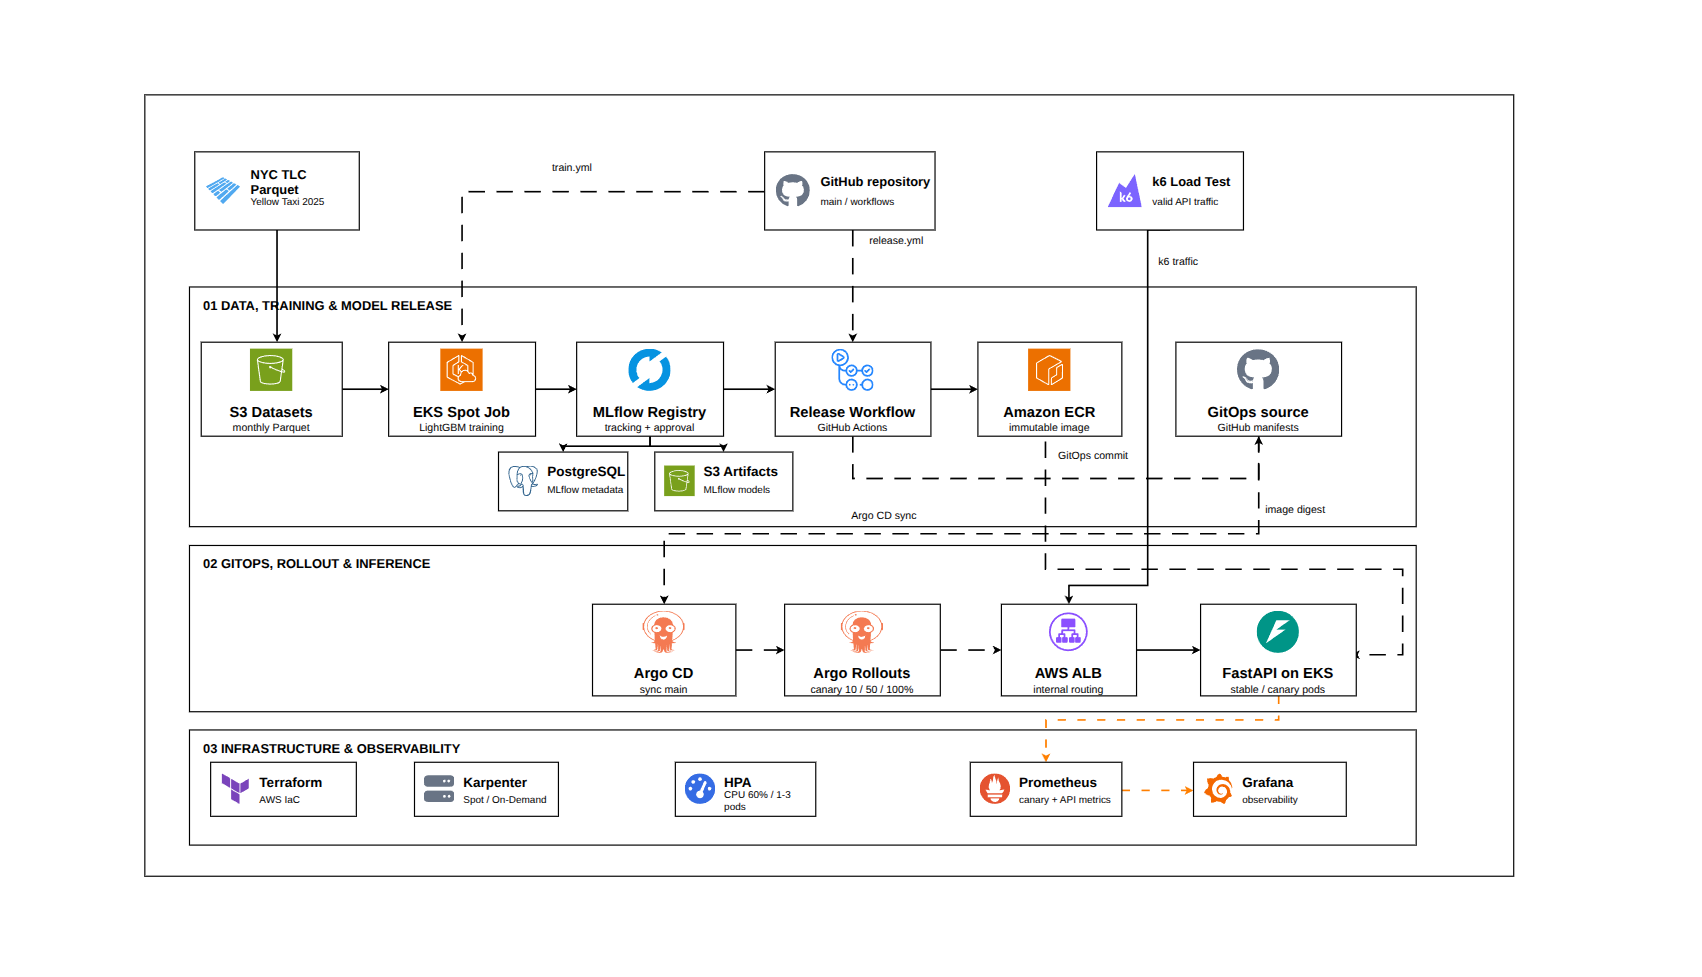
\includegraphics[width=\linewidth,height=0.43\textheight,keepaspectratio,trim={140.00000bp 95.00000bp 185.00000bp 90.00000bp},clip]{Pictures/architecture.png}
\caption{Kiến trúc tổng thể nền tảng MLOps trên AWS.}
\label{fig:architecture}
\end{figure}

\subsubsection{Quản lý hạ tầng và vận hành}


Hạ tầng AWS được quản lý bằng Terraform và chia thành ba lớp có vòng đời độc lập:


\begin{itemize}

\item 

\textbf{Bootstrap:} Khởi tạo tài nguyên phục vụ lưu trữ Terraform state.


\item 

\textbf{Persistent:} Quản lý các tài nguyên cần duy trì lâu dài như S3 datasets, model artifacts, backups và ECR.


\item 

\textbf{Platform:} Triển khai VPC, EKS, IAM và các thành phần hạ tầng phục vụ vận hành Kubernetes.


\end{itemize}

Cách tổ chức này cho phép quản lý hoặc dừng môi trường thực nghiệm mà không đồng thời xóa những dữ liệu và artifacts cần được bảo toàn.


Trong EKS, Managed Node Group \code{system} vận hành các dịch vụ nền như MLflow, PostgreSQL và monitoring. Karpenter quản lý hai NodePool riêng biệt: \code{training-spot} dành cho Kubernetes Training Jobs và \code{inference-on-demand} dành cho dịch vụ FastAPI. Việc sử dụng Spot cho workload huấn luyện giúp tối ưu chi phí, trong khi On-Demand được ưu tiên cho dịch vụ dự đoán cần hoạt động ổn định.


Hệ thống sử dụng GitHub Actions để thực hiện các workflow kiểm thử, huấn luyện và phát hành. Các workflow truy cập AWS thông qua OIDC kết hợp IAM Role, với quyền hạn được phân tách theo nhiệm vụ.


Đối với ứng dụng serving, GitOps được sử dụng để quản lý trạng thái triển khai. Argo CD theo dõi cấu hình Kubernetes trong repository và đồng bộ các thay đổi lên EKS. Argo Rollouts điều phối quá trình cập nhật phiên bản, trong khi ALB phân phối yêu cầu giữa hai Kubernetes Service: \code{inference-api} (stable) và \code{inference-api-canary} (candidate).


Các thành phần giám sát hoạt động song song với dịch vụ dự đoán. Prometheus thu thập request metrics và latency từ FastAPI; Grafana hỗ trợ trực quan hóa các chỉ số. Metrics Server cung cấp dữ liệu CPU cho Horizontal Pod Autoscaler (HPA), cho phép điều chỉnh số lượng Pod phục vụ theo tải.


Trong kiến trúc này, \textbf{HPA điều chỉnh số Pod của Rollout}, còn Karpenter quản lý tài nguyên EC2 node. Hai cơ chế phối hợp nhưng đảm nhiệm những cấp độ mở rộng khác nhau.


\subsection{Luồng dữ liệu và vòng đời mô hình}


Hệ thống tổ chức vòng đời mô hình thành hai quy trình chính: \textbf{huấn luyện và kiểm duyệt mô hình}, sau đó \textbf{phát hành và giám sát phiên bản phục vụ}. Hai quy trình được tách biệt nhằm bảo đảm mô hình đạt yêu cầu về chất lượng dự đoán trước khi được đánh giá khả năng vận hành.


\begin{figure}[!htbp]\centering
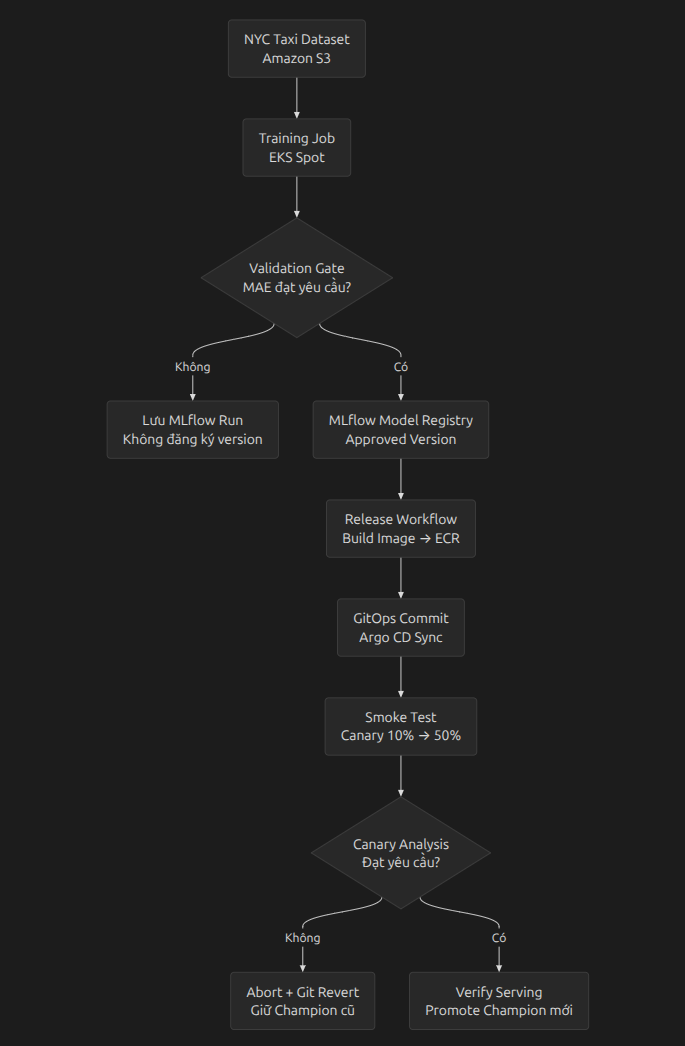
\includegraphics[width=0.86\linewidth,height=0.62\textheight,keepaspectratio]{Pictures/lifecycle.png}
\caption{Luồng dữ liệu và vòng đời mô hình MLOps.}
\label{fig:lifecycle}
\end{figure}

\subsubsection{Huấn luyện và quản lý mô hình}


Dữ liệu NYC Taxi được kiểm tra và lưu trên Amazon S3. Khi Training workflow được kích hoạt, Kubernetes Job trên Spot node thực hiện tiền xử lý, huấn luyện LightGBM và ghi nhận kết quả vào MLflow. Metadata được lưu trong PostgreSQL, còn model artifacts được lưu trên S3.


Sau huấn luyện, \textbf{Validation Gate} so sánh chất lượng candidate với mô hình tham chiếu trên cùng tập validation. Nếu không đạt yêu cầu, kết quả thí nghiệm vẫn được lưu nhưng không tạo phiên bản Registry mới. Ngược lại, candidate đạt yêu cầu sẽ được đăng ký và phê duyệt trong MLflow Model Registry.


Quy trình huấn luyện không tự động triển khai mô hình hoặc thay đổi alias \code{champion}. Việc cập nhật phiên bản phục vụ được kiểm soát thông qua Release workflow độc lập.


\subsubsection{Phát hành và kiểm soát phiên bản phục vụ}


Release workflow tiếp nhận một phiên bản mô hình đã được phê duyệt, xác minh thông tin và đóng gói model cùng ứng dụng FastAPI thành Docker image. Image được lưu trên Amazon ECR và tham chiếu bằng digest trong GitOps manifests. Argo CD đồng bộ cấu hình mới, sau đó Argo Rollouts điều phối quá trình triển khai.


Trước khi nhận lưu lượng, candidate phải vượt qua bước kiểm tra trạng thái và danh tính bản phát hành. Hệ thống tiếp tục phân chia traffic qua ALB theo các mức \textbf{10\% → 50\%}, đồng thời sử dụng Prometheus để đánh giá tỷ lệ lỗi HTTP 5xx, P95 latency và lưu lượng đến candidate.


Khi các điều kiện được đáp ứng, phiên bản mới được promotion và workflow xác minh trạng thái phục vụ trước khi cập nhật alias \code{champion}. Nếu candidate bị từ chối, Argo Rollouts thực hiện abort, đưa traffic trở lại stable; workflow tiếp tục hoàn nguyên thay đổi GitOps có kiểm soát và giữ nguyên phiên bản champion trước đó.


Cơ chế này hình thành \textbf{hai lớp kiểm soát độc lập}: Validation Gate đánh giá chất lượng mô hình, còn Canary Analysis đánh giá khả năng vận hành khi triển khai. Cơ chế rollback tự động hiện được áp dụng cho trường hợp candidate bị từ chối theo các điều kiện xác định, không bao phủ mọi tình huống lỗi của workflow.


\par\medskip\noindent\rule{\linewidth}{0.3pt}\par\medskip

Kiến trúc trên là cơ sở để triển khai các thành phần hạ tầng, huấn luyện và phục vụ mô hình. Cách hiện thực cụ thể được trình bày trong Chương 3, trong khi kết quả kiểm chứng và đánh giá hệ thống được tập trung tại Chương 4.

